% -*-cap1.tex-*-
% Este fichero es parte de la plantilla LaTeX para
% la realización de Proyectos Final de Carrera, protejido
% bajo los términos de la licencia GFDL.
% Para más información, la licencia completa viene incluida en el
% fichero fdl-1.3.tex

% Copyright (C) 2009 Pablo Recio Quijano 

%\section{Introducción}

A continuación se muestran los resultados del estudio tal y como se describieron en la sección anterior.

\section{Localización de la literatura}
En la tabla \ref{tab:ResumenBusquedaResultados} se muestran las búsquedas realizadas en las bibliotecas digitales más importantes en ciencias de la computación, los términos de búsqueda utilizados y el número de documentos obtenidos. Se realizarion numerosas pruebas de búsqueda, ya que los resultados obtenidos cuando el filtrado era muy riguroso menguaba de manera considerable. Sin embargo, relajar el filtro suponía la proliferación de literatura relacionada muy vagamente con nuestro ámbito de investigación. Esto es así porque en prácticamente todos los ámbitos de la ciencia se está fomentando el desarrollo de competencias genéricas, sin embargo, no todos los estudios abordan su evaluación, y mucho menos lo hacen de manera automizada. Realizar la búsqueda por el término "Assessment of generic skills" o "assessing generic skills" nos planteaba la primera problemática, y es que el número de artículos para devueltos era muy reducido. Sin embargo, debilitando la búsqueda con términos como "generic competences" o "generic skills" junto con la palabra "assessment" daba un número de resultados muy elevado. Por esto, finalmente se optó por añadir a esta segunda casuística nomenclatura relacionada con la evalación asistida por ordenador: TEL (Technology Enhanced Learning), ICT (Information and communications technology), CBI (computer-based instruction), o LMS (Learning Managment System). En cada biblioteca, se utilizaron los formularios de búsqueda avanzada.

\begin{table}[H]
  \begin{center}
  \begin{tabular}{| m{3.5cm} | m{6cm} | m{3cm} | c |}
    \hline
    SOURCE & SEARCH TERMS & SEARCH SCOPE & RESULTS\\
    \hline
    \hline
    Wiley Online Library & assessment AND ``generic competences`` OR ``generic skills`` AND (TEL OR ICT OR CBI) & in All Fields & 140 \\
    \hline
    World Scientific Net & ``generic competences`` OR ``generic skills`` AND assessment & Anywhere in article & 20\\
    \hline
    Springer & (``generic skills`` OR ``generic competences``) AND  students AND (TEL OR CBI OR ICT) & All fields (Including full text) & 141\\
    \hline
    ACM Digital Library & (assessment and ``generic skills``) and (TEL or LMS or ICT or CBI) & Any field (title, abstract, review) & 57\\
    \hline
    ACM Digital Library & (assessment and ``generic competences``) and (TEL or LMS or ICT or CBI) & Any field (title, abstract, review) & 15\\
    \hline
    IEEE Digital Library (Xplore) & (((TEL or LMS or ICT or CBI) AND (``generic skills`` OR ``generic competences``)) AND assessment) & Full text and metadata & 48\\
    \hline
    Scopus & (((TEL or LMS or ICT or CBI) AND (``generic skills`` OR ``generic competences``)) AND assessment) & All fields (Including full text) & 47\\
    \hline
    \multicolumn{3}{|r|}{TOTAL} & 467\\
    \hline
  \end{tabular}
\end{center}
\caption{Bibliotecas digitales utilizadas, palabras de búsqueda utilizadas en cada uno y número de resultados obtenidos}
\label{tab:ResumenBusquedaResultados}
\end{table} 


%\section{Selección de trabajos}
%En la tabla \ref{tab:ResumenSelecccionResultados} se muestran los resultados de la clasificación.

En total se recopilaron 468 trabajos, que fueron revisados para identificar si eran de utilidad para el estudio y descartados si cumplían alguno de los criterios de exclusión. El número de estudios primarios resultante (después de aplicar criterios de selección y exclusión) fue de sólo 32 trabajos (casi un 7\% del total de trabajos recopilados). Aunque hay muchos trabajos que tratan las competencias genéricas desde diferentes perspectivas, son muy pocos los que abordan su evaluación desde el punto de vista de la tecnología. De ahí estos resultados, cuya primera y optimista interpretación es que pudiera haber un nicho de investigación. Los resultados de esta clasificación pueden verse e la tabla \ref{tab:ResumenSelecccionResultados}.

\begin{table}[H]
  \begin{center}
  \begin{tabular}{| m{4cm} | c | c |}
    \hline
    CRITERION & STUDIES & FRECUENCY\\
    \hline
    \hline 
    Included & 32 & 6,84\% \\
    \hline
    Off Topic & 407 & 86,97\% \\
    \hline
    Unsupported Language & 1 & 0,21\% \\
    \hline
    Duplicated & 20 & 4,27\% \\
    \hline
    Unread & 8 & 1,71\% \\
    \hline
    Total & 468 & 100\% \\
    \hline
  \end{tabular}
\end{center}
\caption{Clasificación de trabajos una vez aplicados los criterios de selección y exclusión}
\label{tab:ResumenSelecccionResultados}
\end{table} 


%\section{Extracción de los datos}
%Se han seleccionado como estudio primario únicamente 37 artículos, un 7,92\% del total de los revisados. Casi la mayor parte de los seleccionados se pueden localizar en los últimos años, entre 2008 y 2013 (Tabla \ref{tab:ResumenAniosResultados} y figura \ref{fig:PublicacionesAnuales}). 

Aunque hace varios años desde que las tecnologías entraron a formar parte de la vida académica, no es hasta 2010, con lo que la Comisión Europea llama la tercera generación de herramientas, cuando se comienzan a integrar la evaluación en las herramientas de aprendizaje, y conceptos como "Data Mining and analysis", "Behavioural tracking" and "Learning analytics" comienzan a asomar \cite{Redecker:2013}. Con esta introducción, damos sentido a la distribución de la producción de la selección primaria a lo largo de los años, que puede verse tanto en la tabla \ref{tab:ResumenAniosResultados} como en la figura \ref{fig:PublicacionesAnuales}. Casi la mayor parte de los seleccionados se pueden localizar en los últimos años, entre 2011 y 2013.


\begin{table}[H]
  \begin{center}
  \begin{tabular}{| m{4cm} | c |}
    \hline
    YEAR & RESULTS\\
    \hline    
    \hline
    2003 & 0\\
    \hline
    2004 & 0\\
    \hline
    2005 & 0\\
    \hline
    2006 & 2\\
    \hline
    2007 & 1\\
    \hline
    2008 & 6\\
    \hline
    2009 & 1\\
    \hline
    2010 & 2\\
    \hline
    2011 & 5\\
    \hline
    2012 & 5\\
    \hline
    2013 & 10 \\
    \hline
  \end{tabular}
\end{center}
\caption{Cantidad de trabajos publicados cada año}
\label{tab:ResumenAniosResultados}
\end{table} 

\begin{figure}[H]
  \begin{center}
    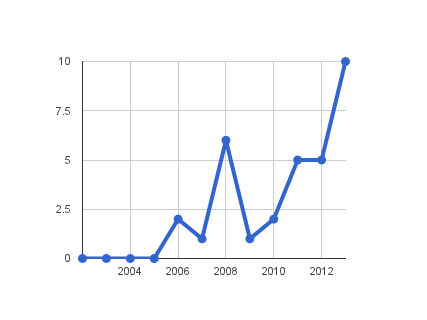
\includegraphics[scale=0.7]{cap3_pub_anuales.png}
  \end{center}
  \caption{Distribución de las publicaciones por años}
  \label{fig:PublicacionesAnuales}
\end{figure}

La revista es el medio en el que más de este tipo de artículos se han publicado, tal y como se puede consultar en la tabla \ref{tab:ResumenForumResultados} y en la figura \ref{fig:PublicacionesTipos} con un 53,1\% del total. Esta información se complementa con la distribución de las publicaciones según el foro en el que han sido publicados y que se muestra en la tabla \ref{tab:DistribucionPublicaciones}. En este se puede comprobar como la mayor parte de las publicaciones están relacionadas con la ingeniería y la educación: World Scientific and Engineering Academy and Society Conferences (WSEAS), IEEE Global Engineering Education Conference (EDUCON), European Journal of Education o Revista Iberoamericana de Tecnologías del Aprendizaje (RITA), entre otras, son las publicaciones que más trabajos han aportado a nuestro trabajo.

\begin{table}[H]
  \begin{center}
  \begin{tabular}{| m{4cm} | c |}
    \hline
    PUBLICATION TYPE & RESULTS\\
    \hline
    \hline 
    Journal & 18 \\
    \hline
    Conference & 10 \\
    \hline
    Chapter & 5 \\
    \hline
  \end{tabular}
\end{center}
\caption{Cantidad de trabajos según el medio en el que fueron publicados}
\label{tab:ResumenForumResultados}
\end{table} 

\begin{figure}[H]
  \begin{center}
    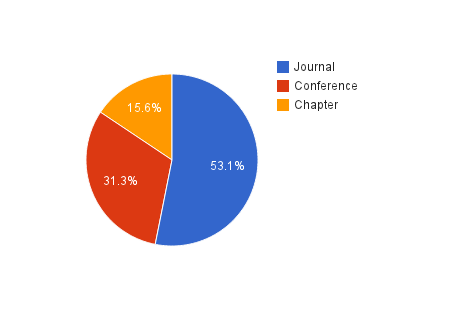
\includegraphics[scale=0.7]{cap3_pub_types.png}
  \end{center}
  \caption{Distribución de publicaciones según el medio en el que fueron publicados}
  \label{fig:PublicacionesTipos}
\end{figure}

\begin{table}[H]
  \begin{center}
  \begin{tabular}{| m{12cm} | c |}
    \hline
    PUBLICATION FORUM & PAPERS\\
    \hline
    \hline 
    World Scientific and Engineering Academy and Society Conferences & 4\\
    \hline
    IEEE Global Engineering Education Conference & 2\\
    \hline
    Australian Society for Computers in Learning in Tertiary Education & 2\\
    \hline
    European Journal of Education & 2\\
    \hline
    Revista Iberoamericana de Tecnologías del Aprendizaje & 2\\
    \hline
    Assessment \& Evaluation in Higher Education & 1\\
    \hline
    Australasian Journal of Educational Technology & 1\\
    \hline
    Conference on Software Engineering Education and Training & 1\\
    \hline
    Competency-based Language Teaching in Higher Education & 1\\
    \hline
    Computers in Human Behavior & 1\\
    \hline
    Computing Colombian Conference & 1\\
    \hline
    Decision Support Systems & 1\\
    \hline
    Game-based learning in higher education and lifelong learning: bridging the gap between theory and practice & 1\\
    \hline
    Human Factors and Ergonomics in Manufacturing \& Service Industries & 1\\
    \hline
    International Conference on Advanced Learning Technologies & 1\\
    \hline
    International Journal of Learning Technology & 1\\
    \hline
    Journal of Computer Assisted Learning & 1\\
    \hline
    Medical Education & 1\\
    \hline
    Revista de Educación & 1\\
    \hline
    The Internet and Higher Education & 1\\
    \hline
    Ubiquitous and Mobile Learning in the Digital Age & 1 \\
    \hline
  \end{tabular}
\end{center}
\caption{Distribución de las publicaciones}
\label{tab:DistribucionPublicaciones}
\end{table} 



\section{Esquema de clasificación y mapeo del estudio}

Una vez revisados todos los artículos se han extraído unas características o categorías comunes a la tipología de los trabajos. Todos los trabajos seleccionados hacen uso de algún tipo de software o metodología para evaluar algún tipo de competencia genérica. Pero ningún trabajo utiliza un enfoque como el que se propone en la introducción de este capítulo, es decir, aprovechando los registros de interacción de los estudiantes con el LMS como indicadores del desempeño de las competencias genéricas. Encontramos trabajos que se apoyan en la tecnología para las competencias pero que terminan delegando parte de la evaluación en el alumno, ya sea mediante autoevaluación o evaluación entre iguales. Otros trabajos se basan en videojuegos o en las redes sociales para evaluar alguna competencia, mientras que otros desarrollan algún tipo de software o técnica. Finalmente hay algunos trabajos que simplemente detectan en su entorno la necesidad de la evaluación de las competencias de manera automática porque su forma de hacerlo les ocasiona una serie de problemas o desventajas con respecto a otro método que proponen o demandan. Además se han encontrado algunas revisiones sobre la literatura relacionadas que también serán tratadas a parte.  En la tabla \ref{tab:PublicacionesForum} se puede ver la distribución de las publicaciones, apoyadas gráficamente en la figura  \ref{fig:PublicacionesForum}. 

\begin{table}[H]
  \begin{center}
  \begin{tabular}{| m{10cm} | c |}
    \hline
    PUBLICATION ISSUE & PAPERS\\
    \hline
    \hline 
    Course’s Learning Outcomes (CLO) and rubrics & 7\\
    \hline
    Peer and self eAssessment & 14\\
    \hline
    Game-Based Learning (GBL) & 6\\
    \hline
    eAssessment and reviews & 5\\
    \hline
  \end{tabular}
\end{center}
\caption{Distribución de publicaciones por tratamiento del problema}
\label{tab:PublicacionesForum}
\end{table} 

\begin{figure}[H]
  \begin{center}
    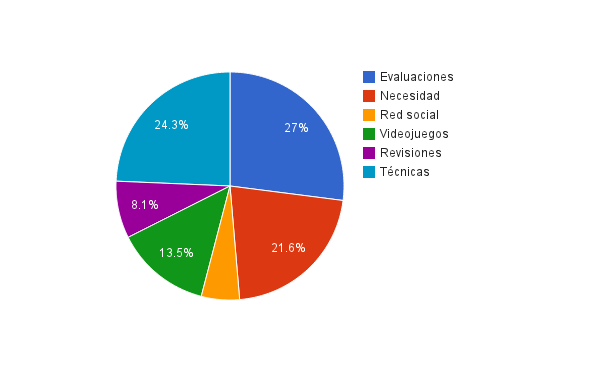
\includegraphics[scale=0.7]{cap3_pub_forum.png}
  \end{center}
  \caption{Distribución de publicaciones por tratamiento del problema}
  \label{fig:PublicacionesForum}
\end{figure}

% Incluir burbujas

La distribución de los trabajos clasificados según su ámbito y su tipo por una lado, y según su ámbito y su contribución por otro, se puede ver en la figura \ref{fig:Burble}.
\begin{landscape}
\begin{figure}[H]
  \begin{center}
    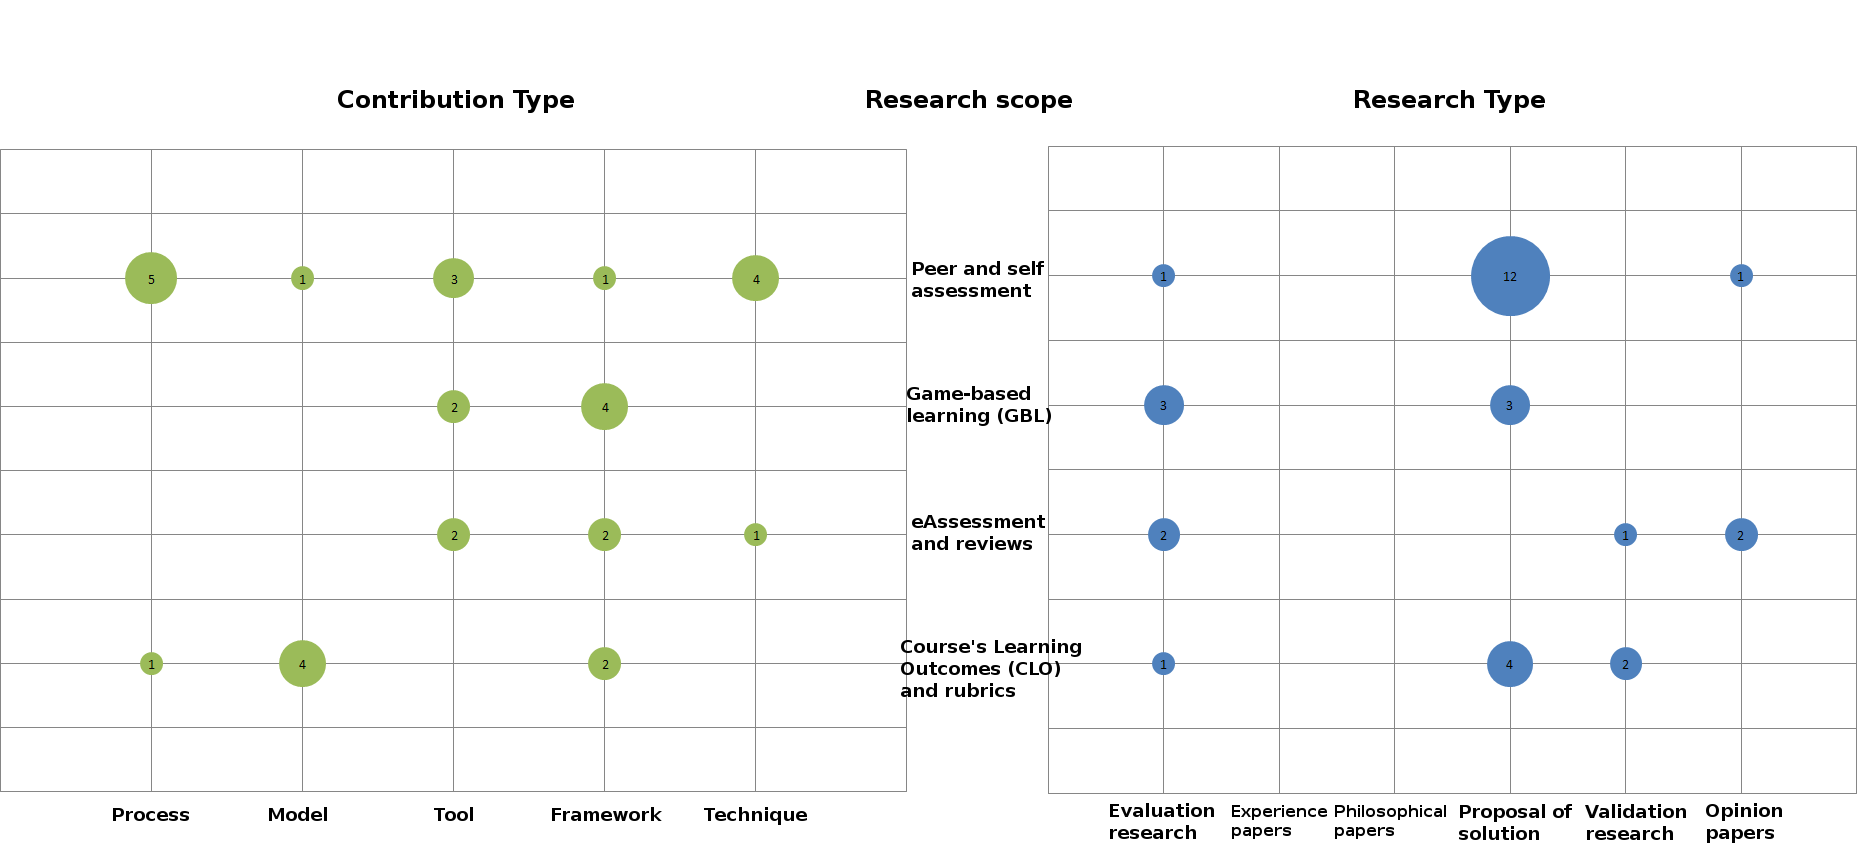
\includegraphics[scale=0.38]{cap3_burbujas.png}
  \end{center}
  \caption{Ámbito de trabajos distribuidos según tipo de investigación y según tipo de contribución.}
  \label{fig:Burble}
\end{figure}
\end{landscape}


\section{Esquema de clasificación}

En los apartados siguientes, se presentan los resultados del estudio para cada área de investigación. El listado de trabajos se muestra en la tabla \ref{tab:ListadoTrabajos}.

\subsection{Course’s Learning Outcomes (CLO) and rubrics}
Hoy en día, las universidades y las empresas van cada vez más de la mano en cuánto hablamos de competencias. Y así ocurre en numerosos artículos de los encontrados en este mapeado cuando se trata de buscar el desarrollo y evaluación de competencias. Y esto es así porque los empresarios buscan profesionales capaces de renovar constantemente sus conocimientos y competencias. Ser capaces de desarrollar y evaluar competencias se convierte, por tanto, en fundamental dentro del nuevo paradigma educativo que emerge del proceso de Bolonia. En este apartado se presentan trabajos que utilizan plantillas generales para las competencias genéricas como una herramienta útil que proporciona información sobre el desarrollo y la evaluación de cada habilidad, con diferentes tipos de matrices de valoración y las plantillas de evaluación. En \cite{Terron-Lopez:2013} se introducen habilidades de empleo genéricos en los programas de los estudiantes de educación superior y son evaluadas medante plantillas de evaluación, mientras que en \cite{Feldt:2009} se echa en falta una evaluación de competencias genéricas y se proponen este tipo rúbricas para ello.

Siguiendo con el ámbito empresarial, nos topamos con el Consorcio RH-XML, una organización independiente y sin ánimo de lucro, dirigido por voluntarios dedicada al desarrollo y promoción de un conjunto estándar de especificaciones para que el comercio electrónico y la automatización de los intercambios de datos relacionadas con recursos humanos. En \cite{Adelsberger:2008} proponen \emph{HR-XML Competencies} con el fin de medir características que sirven como indicadores de competencias. Se pretende establecer unos valores estándares para integrarlos en los recursos del consorcio.

% \cite{SimonTaylor:2009, Anderson:2001,Kennedy:2007} NO FORMAN PARTE DE ESTUDIO. SOLO SON REFERENCIAS 
Por otro lado, cuando hablamos de \emph{Course’s Learning Outcomes (CLO)} nos referimos a objetivos de aprendizaje que describen con claridad las competencias que un estudiante debe poseer al completar el curso \cite{SimonTaylor:2009, Anderson:2001,Kennedy:2007}. En \cite {Mohamed:2008,Mohamed:2008a,Rashid:2008} se implementan diversos modelos para mediante diferentes indicadores valorar el desempeño de los estudiantes en las competencias. En \cite{MercedesRico:2013} partiendo de metodologías de aprendizaje social y colaborativo, utilizando las plataformas de gestión como Moodle, las redes sociales y Second Life, se presenta un trabajo que tiene como objetivo presentar un conjunto de estrategias de enseñanza, tareas y prácticas para desarrollar las competencias transversales necesarias para el estudio tanto éxito y futura integración profesional. Se evalúan las competencias de liderazgo, trabajo en equipo y razonamiento crítico mediante el uso de rúbricas y la corrección de varios profesores.

En resumen, se puede decir que estos trabajos tratan la evaluación de competencias mediante el uso de rúbricas, estableciéndose unos indicadores que marcarán en éstos si los alumnos o el personal a evaluar ha alcanzado el desempeño en éstas. Aunque pueden servir como referencia a la hora de evaluar competencias genéricas, estos sistemas no están integrados en las herramientas de evaluación, y aún estándolos, no liberan al docente de la carga que supone la corrección o revisión de dichas rúbricas.

\subsection{Peer and self eAssessment}

En muchos trabajos se fomenta el uso de alguna herramienta de tipo \emph{portfolio} o diario de aprendizaje, incluídas en los LMS actuales. Estos se han convertido en una ventana que proporciona información del trabajo del estudiante y permite conocer su forma de pensar \cite{Palomares:2011,Gil:2011}. A posteriori son los compañeros o los propios estudiantes los que deben evaluar su evolución y analizar si han conseguido o mejorado ciertas competencias genéricas. Igualmente ocurre en \cite{Lim:2011}, donde los estudiantes trabajan en grupo en un wiki y posteriormente evalúan las competencias de sus compañeros mediante el uso de una rúbrica. Otro tipo de estrategia con una idea parecida se utilizan en la evaluación entre iguales es la integración de los entornos de aprendizaje con las redes sociales \cite{Piedra:2010,McLoughlin:2006,Shih:2011}. Los profesores proporcionan rúbricas que permiten a los estudiantes entender las expectativas de sus instructores. Los alumnos proporcionan información directa a sus compañeros acerca de lo que han aprendido y lo que todavía tienen que aprender. En segundo lugar, los compañeros o ellos mismos pueden usar las rúbricas para la auto-evaluación. 

Una experiencia muy similar pero utilizando herramientas multimedia es la que se lleva a cabo en otro grupo de trabajos. Uno de ellos es el proyecto mostrado en \cite{Martin-Cuadrado:2013}, donde se realizan videoconferencias entre estudiantes de una universidad española y otra estadounidense. Así se pretende promover un aprendizaje autónomo y la mejora de la competencia de comunicación en un segundo idioma. Otro trabajo es el realizado en \cite{Masip-Alvarez:2013}, donde mediante autograbación se evalúan ciertas competencias genéricas. Los alumnos son divididos en grupos por el profesor, se graban en vídeo, se cuelgan en el campus y se auto-corrigen viendo sus fallos y mejorándolos. Son dos experiencias en las que los alumnos corrigen sus propios trabajos y son capaces de valorar si han alcanzado o no ciertas competencias a partir de su evolución.

Otros artículos en los que se trabaja también con la autoevaluación son \cite{Colomo-Palacios:2013,Liao:2013,McMahon:2007,Murdoch-Eaton:2012,Chebil:2012,Cardona:2013}. Con este grupo de trabajos se soluciona el problema de escalalabilidad con la autoevaluación o evaluación entre iguales. Sin embargo, la calificación depende en gran medida de la subjetividad del alumno y una revisión minicuiosa del profesor seguiría siendo un trabajo poco escalable. 

\subsection{Game-Based Learning (GBL)} 
La aplicación de los conocimientos teóricos a la práctica es uno de los objetivos más importante y hacia esta dirección apuntan diversos métodos y enfoques que se han desarrollado. Un aprendizaje significativo incrustado en la experiencia es difícil de proporcionar dentro de los planes de estudios regulares. Sería ideal poder trabajar sobre situaciones de la vida real, y poder integrar este tipo de experiencias en los planes de estudios universitarios sin riesgos. En varios trabajos se muestra la integración de los entornos de trabajo auténticos con el fin de apoyar la aplicación práctica de los conocimientos teóricos dentro de los enfoques de enseñanza y aprendizaje en los cursos de postgrado y formación permanente. Estas experiencias se llevan a cabo con simulaciones y juegos \cite{Petersen:2012,Borrajo:2010}.

Los \emph{juegos serios} ofrecen nuevos desafíos y oportunidades para el desarrollo de competencias. Este potencial implica cuestiones de investigación complejos, tales como la forma de evaluar las competencias sin perturbar el juego en sí al que se enfrenta el estudiante, así como la forma de diseñar el juego de modo que las competencias pueden ser desarrolladas por los alumnos. A fin de evaluar las competencias, es útil describirlas en términos de la conducta que se observa e interpreta mientras que un estudiante está involucrado en el juego. Sin embargo, la interpretación de estos indicadores de comportamiento en términos de competencias, y en particular, de las habilidades sociales, está mediada por factores contextuales \cite{Bedek:2011}. En otro trabajo basado en un juego serio \cite{Guenaga:2013}, se utiliza una aventira gráfica mediante la que los alumnos desarrollan y evaluan sus propias competencias de espíritu empresarial y resolución de problemas.

Otra herramienta de simulación es VIRBUS \cite{Starcic:2008,Starcic:2008a}. VIRBUS un juego que simula un problema de la vida real y ayuda evaluar la competencia genérica de \emph{resolución de problemas} mediante la salida esperada al problema y la encontrada por el alumno (o grupo de alumnos). El objetivo principal de la aplicación de esta herramienta es facilitar el aprendizaje autodirigido del estudiante. Además, los estudiantes obtienen retroalimentación, no sólo una evaluación de sus resultados de aprendizaje.

Los juegos ofrecen mecanismos para desarrollar y evaluar las competencias de sus estudiantes, y algo muy importante, es que los alumnos aprenden jugando. Aunque nos enfrentamos a varios problemas con respecto a nuestra propuesta. Por un lado, son herramientas que no están integradas en el sistema, por lo que conllevan consigo algún mecanimos manual de traslado de calificaciones. Además, los juegos suelen ir orientados a un reducido grupo de competencias, readaptar el juego para evaluar otra competencias sería algo muy costoso. Y tener varios juegos puede encaminarnos a un nuevo panorama de trabajo poco escalable para el profesor. 


\subsection{eAssessment and reviews}
Este grupo de artículos están más orientados a la tercera generación en las estrategias de evaluación (\emph{eAssessment}), enfocados en minería de datos, seguimiento del comportamiento y análisis integrado de aprendizaje de los estudiantes en lo referente a su interacción con el entorno virtual \cite{Redecker:2012,Redecker:2013}. En los artículos encontrados se realiza una revisión del estado del arte actual y se plantean las bases para nuevas herramientas.

Por último quedan una serie de trabajos que evalúan competencias, y aunque su faceta tecnológica no ha podido ser desgranado con precisión, dada la ausencia de información en el trabajo, sí se puede vislumbrar que se ha apoyado en algún u otro aspecto de la tecnología para su desempeño. En \cite{Velasco:2012} se combinan instrumentos para evaluar a los estudiantes como exámenes tradicionales, sesiones prácticas con ordenador y trabajos en grupos para evaluar la adquisición de competencias. En \cite{Achcaoucaou:2012} se muestra Tripuscoid, una herramienta que, en primer lugar, permite a los estudiantes a identificar sus puntos fuertes y débiles y desarrollar estrategias personales para la mejora, en segundo lugar, proporciona a los profesores información adicional sobre los efectos de su entrada en las competencias de los estudiantes, y por último, proporciona información útil para gestión de la calidad de los programas de enseñanza, ya que puede detectar necesidades de formación de los nuevos estudiantes y ayudar a mejorar el contenido y diseño de los futuros programas académicos. En \cite{BenoCsap:2012} se examinan algunos casos especiales para los que las nuevas tecnologías han permitido avances significativos (por ejemplo, las evaluaciones de los alumnos con necesidades educativas especiales, la evaluación de habilidades de colaboración y la consecución de grupo). 

Aunque su aportación es interesante para este trabajo, los métodos presentados distan de las soluciones que necesitamos para tratar los problemas de escalabilidad y subjetividad.

\begin{landscape}
\begin{center}
\begin{longtable}{| c | m{9.5cm} | m{4cm} | m{4cm} | m{4cm} |}
    \hline
    REF & TITLE & RESEARCH SCOPE & RESERACH TYPE & CONTRIBUTION TYPE \\
    \hline
    \hline 
    \cite{Chebil:2012} & An ontology and a software framework for competency modeling and management & & & \\
    \hline
    \cite{Mohamed:2008a} & Appraisal of course learning outcomes using rasch measurement: a case study in information technology education & Course’s Learning Outcomes (CLO) \& rubrics & Evaluation research & Model \\
    \hline
    \cite{Terron-Lopez:2013} & Assessing Transferable Generic Skills in Language Degrees & Course’s Learning Outcomes (CLO) \& rubrics & Solution proposal & Framework \\
    \hline
    \cite{McLoughlin:2006} & Beyond marks and measurement: Developing dynamic and authentic forms of e-assessment & Peer \& self eAssessment & Solution proposal & Technique \\
    \hline
    \cite{Shih:2011} & Can Web 2.0 technology assist college students in learning English writing? Integrating Facebook and peer assessment with blended learning & Peer \& self eAssessment & Solution proposal & Technique  \\
    \hline
    \cite{Petersen:2012} & Challenges and opportunities in evaluating learning in serious games: a look at behavioural aspects & Game-Based Learning (GBL) & Solution proposal & Framework\\
    \hline
    \cite{Redecker:2013} & Changing Assessment — Towards a New Assessment Paradigm Using ICT & eAssessment and reviews & Evaluation research & Framework \\
    \hline
    \cite{Achcaoucaou:2012} & Competence Assessment in Higher Education: A Dynamic Approach & eAssessment and reviews & Validation research & Tool \\
    \hline
    \cite{Colomo-Palacios:2013} & Competence gaps in software personnel: A multi-organizational study & Peer \& self eAssessment & Solution proposal & Process \\
    \hline
    \cite{Adelsberger:2008} & Competence Models in Technology-Enhanced Competence-Based Learning & Course’s Learning Outcomes (CLO) \& rubrics & Solution proposal & Model \\
    \hline
    \cite{Gil:2011} & Cooperative learning and electronic group portfolio: tutoring tools, development of competences and assessment & Peer \& self eAssessment & Solution proposal & Technique \\
    \hline
    \cite{Liao:2013} & Developing a diagnosis system of work-related capabilities for students: A computer-assisted assessment & Peer \& self eAssessment & Solution proposal & Process \\
    \hline
    \cite{Velasco:2012} & Developing Generic Competences in the European Higher Education Area: a proposal for teaching the principles of economics & eAssessment and reviews & Evaluation research & Framework \\
    \hline
    \cite{Starcic:2008} & Developing virtual simulation game for authentic learning: realizing partnership between university and industry & Game-Based Learning (GBL) & Validation research & Framework \\
    \hline
    \cite{Redecker:2012} & eAssessment for 21st century learning and skills & eAssessment and reviews & Opinion papers & Technique \\
    \hline
    \cite{Rashid:2008} & Engineering students performance evaluation of generic skills measurement: ESPEGS model & Course’s Learning Outcomes (CLO) \& rubrics & Solution proposal & Model \\
    \hline
    \cite{MercedesRico:2013} & Everything Matters: Development of Cross-Curricular Competences in Engineering Through Web 2.0 Social Objects &  Course’s Learning Outcomes (CLO) \& rubrics & Solution proposal & Process \\
    \hline
    \cite{McMahon:2007} & Explorations in metacognition: The design, development, and implementation of an online teamwork tracking environment & Peer \& self eAssessment & Solution proposal & Tool \\
    \hline
    \cite{Bedek:2011} & From Behavioral Indicators to Contextualized Competence Assessment & Game-Based Learning (GBL) & Validation research & Framework \\
    \hline
    \cite{Starcic:2008a} & Game-based learning in higher education and lifelong learning: bridging the gap between theory and practice & Game-Based Learning (GBL) & Solution proposal & Framework \\
    \hline
    \cite{Murdoch-Eaton:2012} & Generic skills in medical education: developing the tools for successful lifelong learning & Peer \& self eAssessment & Solution proposal & Tool \\
    \hline
    \cite{Feldt:2009} & Generic Skills in Software Engineering Master Thesis Projects: Towards Rubric-Based Evaluation & Course’s Learning Outcomes (CLO) \& rubrics & Validation research & Framework \\
    \hline
    \cite{Martin-Cuadrado:2013} & Innovation Network: Videoconferencing as a Resource in Teaching Support and Autonomous Learning & Peer \& self eAssessment & Evaluation research & Framework \\
    \hline
    \cite{Piedra:2010} & Measuring collaboration and creativity skills through rubrics: Experience from UTPL collaborative social networks course & Peer \& self eAssessment & Solution proposal & Process \\
    \hline
    \cite{Mohamed:2008} & Outcome based education performance measurement: a Rasch-based longitudinal assessment model to measure information management courses LO's & Course’s Learning Outcomes (CLO) \& rubrics & Validation research & Model \\
    \hline
    \cite{Masip-Alvarez:2013} & Self-video recording for the integration and assessment of generic competencies & Peer \& self eAssessment & Solution proposal & Process \\
    \hline
    \cite{Guenaga:2013} & Serious Games for the Development of Employment Oriented Competences  & Game-Based Learning (GBL) & Validation research & Tool \\
    \hline
    \cite{Borrajo:2010} & SIMBA: A simulator for business education and research & Game-Based Learning (GBL) & Solution proposal & Tool \\
    \hline
    \cite{BenoCsap:2012} & Technological Issues for Computer-Based Assessment & eAssessment and reviews & Opinion papers & Tool \\
    \hline
    \cite{Palomares:2011} & The educational model at university and the use of new methodologies for teaching, learning and assessment & Peer \& self eAssessment & Solution proposal & Technique \\
    \hline
    \cite{Cardona:2013} & Towards a model for assessing competencies & Peer \& self eAssessment & Opinion papers & Model \\
    \hline
    \cite{Lim:2011} & Using wikis to develop student teachers' learning, teaching, and assessment capabilities & Peer \& self eAssessment & Solution proposal & Process \\
    \hline
\caption{Distribución de publicaciones por tratamiento del problema}
\label{tab:ListadoTrabajos}
\end{longtable}
\end{center}
\end{landscape}




% En los siguientes apartados, se presentan los resultados del estudio para cada área de investigación. %Los documentos base de este estudio están incluidos en el Apéndice.

% \subsection{Metodologías que delegan en los alumnos}
% Para favorecer el desarrollo del aprendizaje se utilizan estrategias evaluativas como la autoevaluación, la evaluación entre iguales y la coevaluación. Estas aportan beneficios a estudiantes y profesores universitarios, como la mejora de los procesos y productos del aprendizaje, el desarrollo de estrategias interpersonales, la mejora de la capacidad para emitir juicios o el desarrollo de determinadas competencias académicas y profesionales \cite{Ibarra:2012}. Además, cuando el número de alumnos y la cantidad de información a tener en cuenta en la evaluación crecen, evaluar el trabajo de cada estudiante se vuelve un trabajo muy poco escalable \cite{Balderas:2012}.

% Esta estrategia se apoya en el uso de algún tipo de tecnología para trabajar y evaluar una competencia genérica, dejando a posteriori a criterio del alumno la labor de valorar si un compañero o él mismo han alcanzado dicha competencia gracias a la actividad desarrollada. Aunque este enfoque tiene sus beneficios tanto para profesores como para estudiantes, una revisión del profesor podría ser igualmente un trabajo inabarcable.

% \subsection{Videojuegos}
% Son numerosos los estudios que han tratado las ventajas del aprendizaje basado en juegos (GBL, Game-based learning) \cite{Costu:2009,Munoz:2011}. En estos trabajos se presentan juegos de simulación virtual para cursos que fomentan la colaboración de la universidad y la industria. Juegos que simulan situaciones de la vida real para el desempeño de ciertas competencias y que serán útiles para la industria. Las simulaciones son ambientes de aprendizaje complejos y desafiantes que presentan dificultades para los estudiantes, ya que éstos carecen de una comprensión fundamental de los conceptos específicos del dominio, las relaciones y estrategias de resolución de problemas \cite{Kirkley:2004}. Uno de los factores importantes de esta simulación es la configuración de aprendizaje \cite{Thavikulwat:2010}, la alineación de objetivos, los métodos de aprendizaje y evaluación con los resultados de aprendizaje previstos. Esta evaluación es el aspecto que más nos interesa analizar. Aunque no siempre se realiza de manera automática, sino que a menudo se apoya en el uso de algún tipo de rúbrica facilitada por el LMS.
 
% \subsection{Técnicas}
% En esta categoría se recogen todos aquellos trabajos que aporten propuestas automáticas o semiautomáticas para la evaluación de competencias genéricas basados en algún modelo. Son herramientas que permiten a los estudiantes, en primer lugar, identificar sus puntos fuertes y débiles y desarrollar estrategias personales para la mejora. En segundo lugar, proporciona a los profesores con información adicional sobre los efectos de su enseñanza en las competencias de los estudiantes. Y por último, proporciona información útil para gestión de la calidad de los programas de enseñanza, ya que puede detectar tendencias en las necesidades de formación de los nuevos estudiantes y ayudar a mejorar el contenido \cite{Achcaoucaou:2012}.

% \subsection{Necesidades}
% La búsqueda de trabajos relacionados no ha proporcionado muchos resultados directamente relacionados. Sin embargo, aunque no aporten una herramienta concreta, sí hemos encontrado trabajos que detectaban la necesidad de un método, herramienta o modelo para la evaluación de competencias genéricas. Se han añadido a este trabajo los más relevantes de dichos artículos. Este cambio conceptual en el área de la evaluación asistida tiene su motivación en el cambio pedagógico global de conocimiento para el aprendizaje basado en competencias y el reciente énfasis en competencias genéricas, ya que son conscientes de que los cambios en los planes de estudio y en los objetivos del aprendizaje son ineficaces si las prácticas de evaluación siguen siendo las mismas \cite{Cachia:2011, Redecker:2013}.

% \subsection{Revisiones}
% Con las diferentes revisiones de estado del arte encontradas con respecto a la evaluación de competencias genéricas, se evidencia que hay varios modelos y herramientas para el desarrollo y evaluación de de las mismas, que hacen hincapié en los modelos de datos que soportan los diferentes procesos formativos. Así mismo se plantean modelos de evaluación apoyados en criterios y los niveles de competencia que deben ser valorados por todos los participantes en el proceso de aprendizaje \cite{Cardona:2013}.

